\documentclass{standalone}
\usepackage{tikz}
\usetikzlibrary{positioning}

\begin{document}
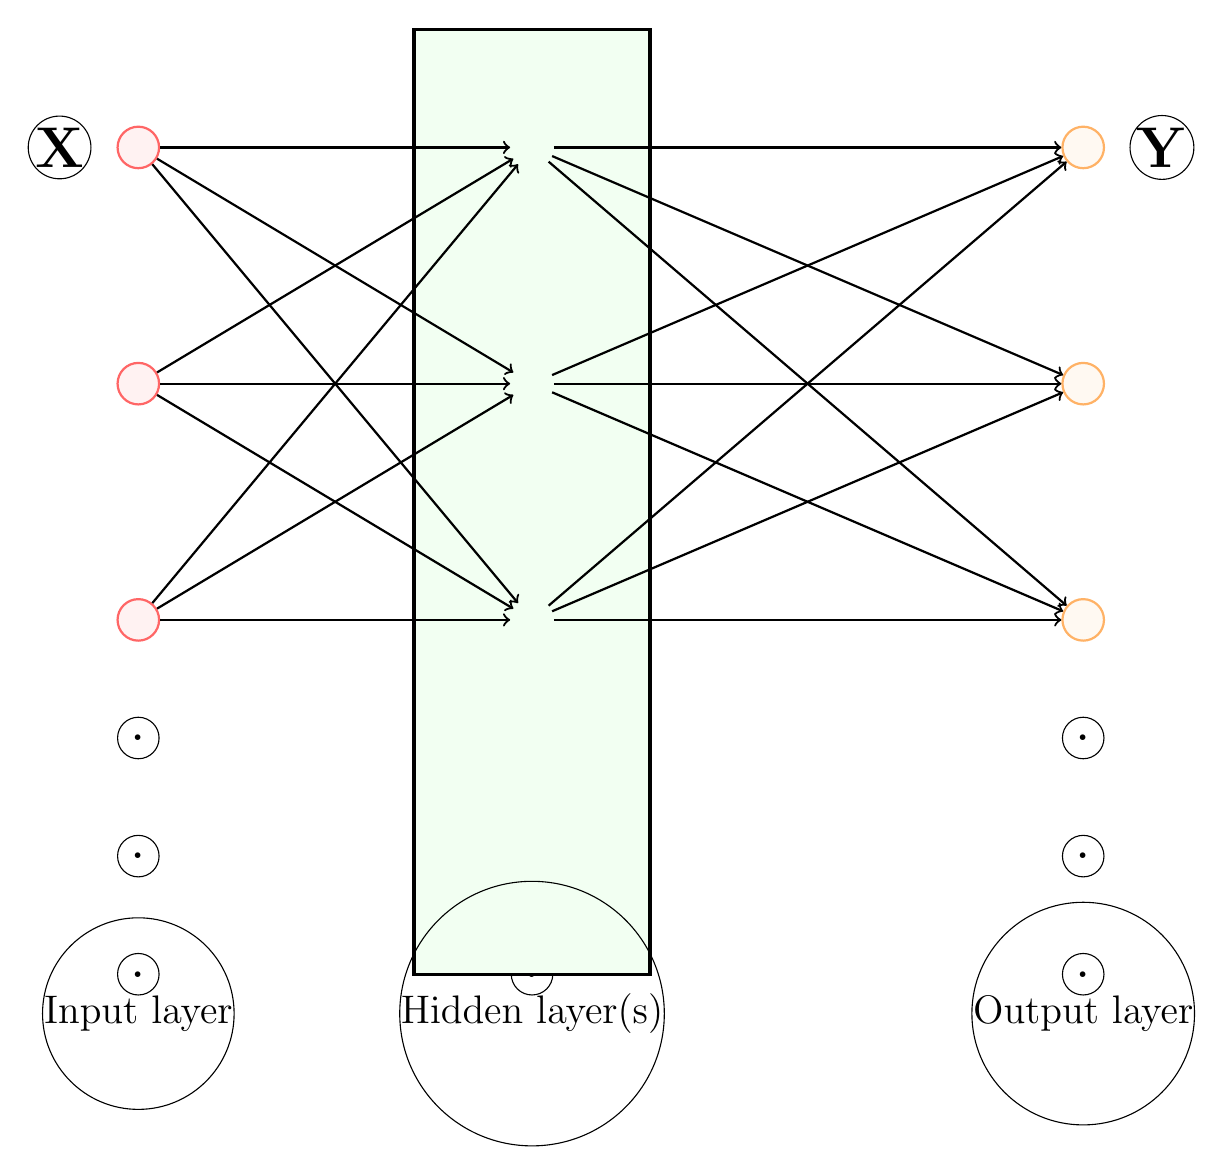
\begin{tikzpicture}[every node/.style={circle, draw, minimum size=1.5em, inner sep=0pt}]

% ===== Define network parameters =====
\def\nInput{3}       % number of input neurons
\def\nHidden{3}      % number of hidden neurons
\def\nOutput{3}      % number of output neurons
\def\ySep{3}         % vertical separation between neurons
\def\xInput{-5}      % x-coordinate input layer
\def\xHidden{0}      % x-coordinate hidden layer
\def\xOutput{7}      % x-coordinate output layer

% ===== Input layer =====
\foreach \i in {1,...,\nInput} {
    \pgfmathsetmacro\y{-(\i-1)*\ySep} % calculate y-position
    \node[fill=red!5, draw=red!60, thick] (I\i) at (\xInput,\y) {};
}
% dots for omitted input neurons
\node at (\xInput, -\ySep*\nInput+0.5*\ySep) {\Huge{.}};
\node at (\xInput, -\ySep*\nInput+0*\ySep) {\Huge{.}};
\node at (\xInput, -\ySep*\nInput-0.5*\ySep) {\Huge{.}};

% ===== Hidden layer =====
\foreach \i in {1,...,\nHidden} {
    \pgfmathsetmacro\y{-(\i-1)*\ySep}
    \node[fill=blue!5, draw=blue!60, thick] (H\i) at (\xHidden,\y) {};
}
% dots for omitted hidden neurons
\node at (\xHidden, -\ySep*\nHidden+0.5*\ySep) {\Huge{.}};
\node at (\xHidden, -\ySep*\nHidden+0*\ySep) {\Huge{.}};
\node at (\xHidden, -\ySep*\nHidden-0.5*\ySep) {\Huge{.}};

% rectangle around hidden layer
\draw[very thick, fill=green!5] (\xHidden-1.5, 1.5) rectangle (\xHidden+1.5, -\ySep*\nHidden-1.5);

% ===== Output layer =====
\foreach \i in {1,...,\nOutput} {
    \pgfmathsetmacro\y{-(\i-1)*\ySep}
    \node[fill=orange!5, draw=orange!60, thick] (O\i) at (\xOutput,\y) {};
}
% dots for omitted output neurons
\node at (\xOutput, -\ySep*\nOutput+0.5*\ySep) {\Huge{.}};
\node at (\xOutput, -\ySep*\nOutput+0*\ySep) {\Huge{.}};
\node at (\xOutput, -\ySep*\nOutput-0.5*\ySep) {\Huge{.}};

% ===== Connections Input → Hidden =====
\foreach \i in {1,...,\nInput} {
    \foreach \j in {1,...,\nHidden} {
        \draw[->, thick] (I\i) -- (H\j);
    }
}

% ===== Connections Hidden → Output =====
\foreach \i in {1,...,\nHidden} {
    \foreach \j in {1,...,\nOutput} {
        \draw[->, thick] (H\i) -- (O\j);
    }
}

% ===== Labels =====
\node at (\xInput, -\ySep*\nInput-2) {\Large{Input layer}};
\node at (\xHidden, -\ySep*\nHidden-2) {\Large{Hidden layer(s)}};
\node at (\xOutput, -\ySep*\nOutput-2) {\Large{Output layer}};

% Optional: network input/output symbols
\node at (\xInput-1,0) {\huge{$\mathbf{X}$}};
\node at (\xOutput+1,0) {\huge{$\mathbf{Y}$}};

\end{tikzpicture}
\end{document}